\section{Functional requirements specification}\label{Functional requirements specification}
Functional requirements specification (FRS) is a document that defines functionality, which application or some parts of application must perform \cite{wiki:frs}. N2Sky is sociotechnical system, meaning that is strongly interacts with humans. 

\subsection{Requirements specifications overview}\label{Requirements specifications overview}

FRS for N2Sky is described in natural language with formal methods in order to establish specifications between development process and end-user consuming. Ever N2Sky module has FRS, which is explicit and points on system functionality. A good FRS must be unambiguous, consistent and correct \cite{frs_1}.  
 
 The formal or semi-formal methods are serving for analysing and validating FRS. The main purpose of  that to limit interpretation errors. The problem occurs when FRS is fully written in natural language, when designers does not have required technical knowledge in order to use other languages. One of  the typical solution is defects detection technics, which require some effort from designer \cite{frs_3}. 
 
In N2Sky some methods and technics were applied in order to make specification clean and clear as possible. Despite that in FRS will be always some parts which are leading to misunderstanding \cite{frs_1}.
  
FRS is a part of engineering phase. Following qualities for N2Sky were defined and applied during this phase \cite{frs_4} as it shown in ``Fig.~\ref{fig:frs_req}'' :
\begin{itemize}
\item Correct
\item Unambiguous
\item Complete
\item Consistent
\item Ranked for importance and/or stability
\item Verifiable
\item Modifiable
\item Traceable 
\end{itemize}


\begin{figure}[htbp]
\begin{center}
  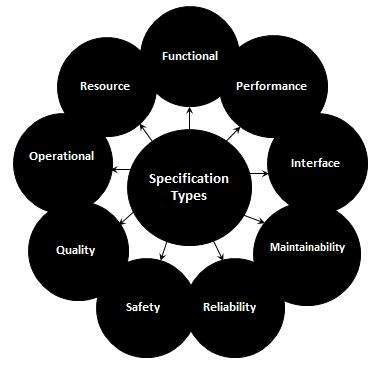
\includegraphics[scale=0.75]{components/4/pics/frs_req.jpg}
  \caption{Applied on N2Sky  Requirement Specification Quialities}
  \label{fig:frs_req}
\end{center}
\end{figure}



\subsection{User Roles}\label{User Roles}

In order to make the N2Sky user interface understandable for arbitrary users as well as professional for advances users, it was decided to separate the user roles. Every user role has own way of interaction with the application:

Every user has some specific area within he works. For example just registered user does not need to know the current environment monitoring information. These restrictions were motivation to create some user roles in order to restrict of grand some functionality of N2Sky as it shown on ``Fig.~\ref{fig:userroles}''.

\begin{figure}[htbp]
\begin{center}
  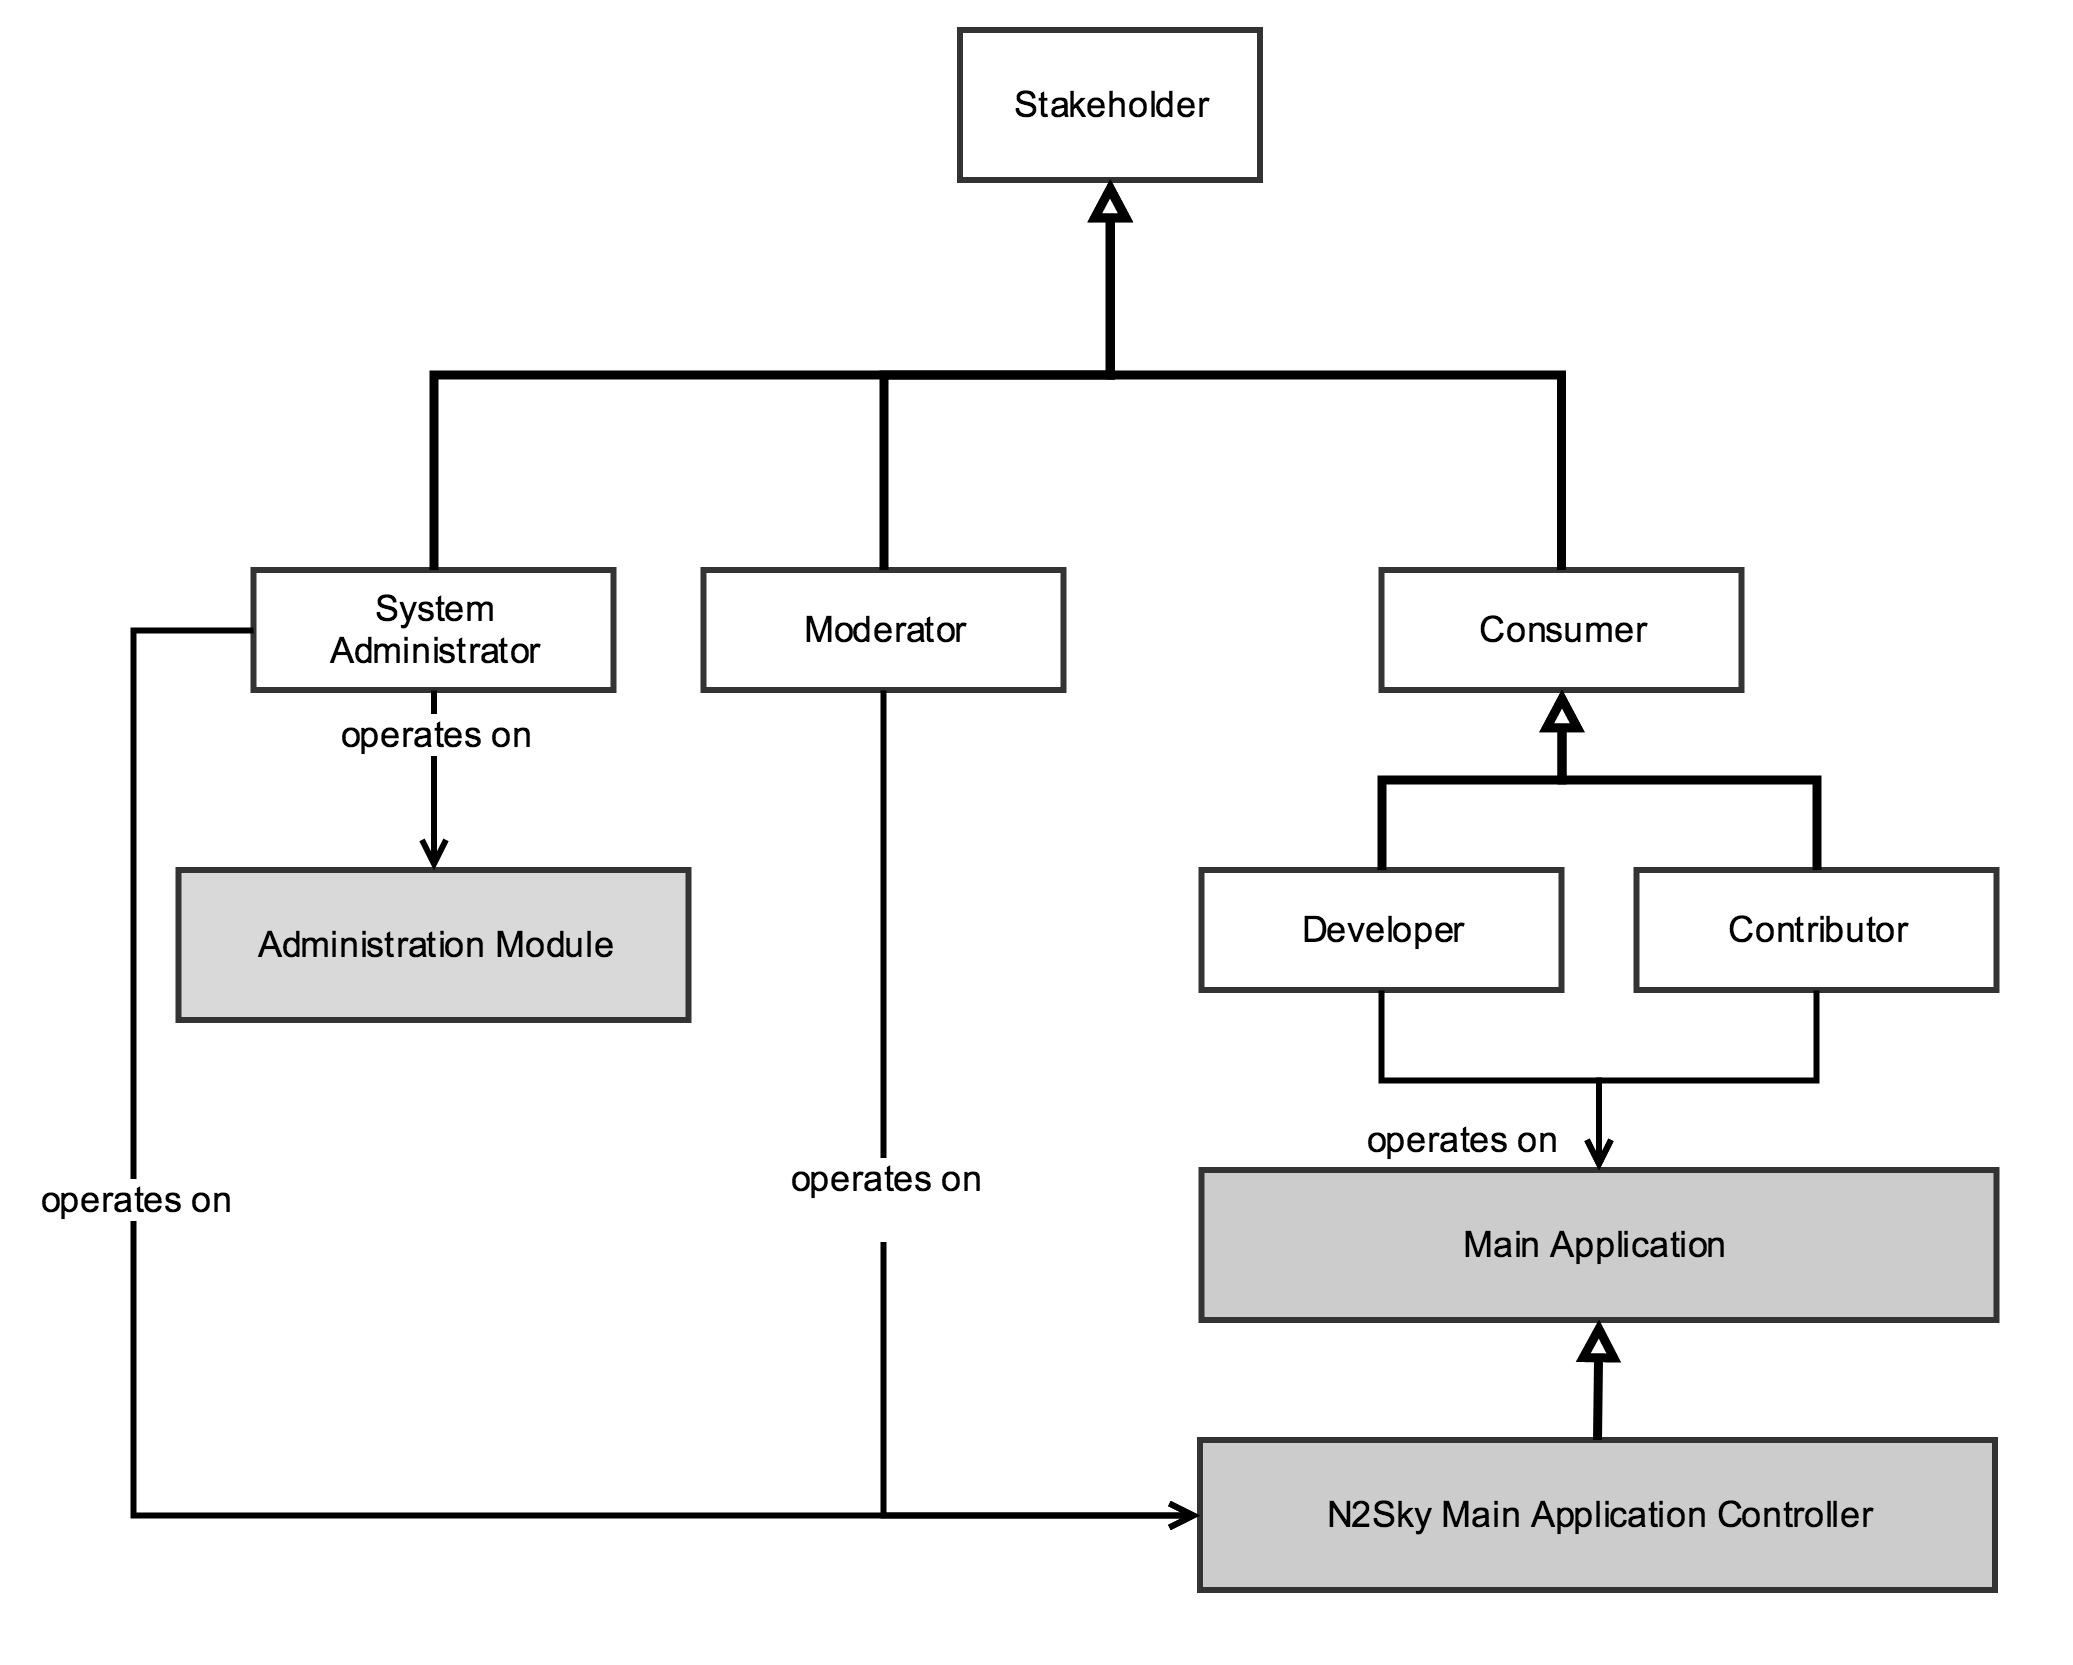
\includegraphics[width=\linewidth]{components/4/users.png}
  \caption{User roles hierarchy and modules where they operating on (marked grey)}
  \label{fig:userroles}
\end{center}
\end{figure}

\begin{description}
\item[Contributor.]   The Contributor is an arbitrary user. Such a user has no necessity in having deep knowledge of the neural network field or know any programming language. The main goal of arbitrary user is to study neural networks within N2Sky. The contributor has access only to his own dashboard and public available resources on the main application module. He can perform semantic search for available neural network paradigms and use them. He can also train running neural network instances and test them. This user can share his trained neural network by making it public. 
\item[Consumer.] The Consumer is an arbitrary user, except he is not creating but using already existing neural networks and trained models. His main purpose is to evaluate trained models or execute training against existing neural networks. This kind of user does not have to use his own training data, he just wants to see the behaviour of neural networks. The Consumer can be converted to Contributor user if he has enough knowledge for it. 
\item[Developer.] The Developer is an expert user, which has enough knowledge and experience to create his own neural network. This user can create neural network paradigms using the ViNNSL schema and publish them on N2Sky. This user can deploy neural networks on the N2Sky environment as well as on his own environment by providing training and testing endpoints. The goal of the developer is the study how his networks will behave with different network structures, input parameters and training data that is provided by other users.
\item[System Administrator.] System Administrator is a user who has a full access to application including environment management, monitoring and alerting features. Administrator can manage Openstack and Cloudify instances. He also can shadow any N2Sky user to observe the application from shadowed user perspective. Administrator has access to all dashboards in every module.
\item[Moderator.] Is a user with a granted permissions. This user can moderate Main Application Module namely neural network instances and  trained models from other users. The Moderator does not have access to Administration Module and can not be converted to System Administrator user role.
\end{description}

\subsection{User Main Functions}\label{User Permissions}

In more detailed overview of user roles it is possible to define permission and main functions.
Permissions describes users allowed page view. If user has access to particular page view the main user function can be defined. 
The main user function characterise allowed behaviour on particular page view. 

As it was mentioned in previous chapter,  N2Sky is an modular application. Permissions and main functions of Administration Module and N2Sky Main Application Controller, which is a part of Main Application Modules, described in Table \ref{table:admin}.

\begin{table}[]
\resizebox{\textwidth}{!}{%
\begin{tabular}{|l|c|c|c|c|c|c|c|c|}
\hline
\multicolumn{1}{|c|}{User Role} & \multicolumn{2}{c|}{\textbf{Administration Module}}          & \multicolumn{2}{c|}{\textbf{N2Sky Main Application Controller}}      \\ \hline
\multicolumn{1}{|c|}{\textbf{}} & \textbf{OpenStack Management} & \textbf{Cloudify Management} & \textbf{Neural Networks Management} & \textbf{Trained Models Management} \\ \hline
System Administrator            & \textbf{+}                    & \textbf{+}                   & \textbf{+}                          & \textbf{+}                            \\ \hline
Moderator                       & \textbf{-}                    & \textbf{-}                   & \textbf{+}                          & \textbf{+}              \\ \hline
Consumer                        & \textbf{-}                    & \textbf{-}                   & \textbf{-}                          & \textbf{-}                            \\ \hline
Developer                       & \textbf{-}                    & \textbf{-}                   & \textbf{-}                          & \textbf{-}                               \\ \hline
Contributor                     & \textbf{-}                    & \textbf{-}                   & \textbf{-}                          & \textbf{-}                    \\ \hline
\end{tabular}%
}
\caption{User Roles main functions considering "Administration Module" and "N2Sky Main Application Controller". 
"+" for allowed, "-" for disallowed}
\label{table:admin}
\end{table}

System Administrator has permissions to all components. Moderator has access only to N2Sky Main Application Controller. Since both of this user roles extending Contributor user role, the permissions for main application module are also granted.

Consumer, Developer and Contributor user roles have no access to any administration parts of N2Sky. This users do not have any main function in this area, but they can operate N2Sky Main Application Module as it shown on Table \ref{table:main}.

\begin{table}[]
\resizebox{\textwidth}{!}{%
\begin{tabular}{|l|c|c|c|c|}
\hline
\multicolumn{1}{|c|}{User Role} & \multicolumn{4}{c|}{\textbf{N2Sky Main Application Module}}                                                                                    \\ \hline
\multicolumn{1}{|c|}{\textbf{}} & \textbf{Paradigm Creation} & \textbf{Neural Networks Creation} & \textbf{Neural Network Training} & \textbf{Training Models Evalutaion} \\ \hline
System Administrator            & \textbf{-}                 & \textbf{-}                        & \textbf{-}                       & \textbf{-}                          \\ \hline
Moderator                       & \textbf{-}                 & \textbf{-}                        & \textbf{-}                       & \textbf{-}                          \\ \hline
Consumer                        & \textbf{-}                 & \textbf{-}                        & \textbf{+}                       & \textbf{+}                          \\ \hline
Developer                       & \textbf{+}                 & \textbf{+}                        & \textbf{+}                       & \textbf{+}                          \\ \hline
Contributor                     & \textbf{-}                 & \textbf{+}                        & \textbf{+}                       & \textbf{+}                          \\ \hline
\end{tabular}%
}
\caption{User Roles main functions considering "N2Sky Main Application Module". 
"+" for allowed, "-" for disallowed}
\label{table:main}
\end{table}

As it was mentioned before System Administrator as well as Moderator has access to N2Sky Main Application Module, but they do not have a main function there. On the other hand all user roles, which are extending consumer can contribute in a N2Sky Main Application Module, except Consumer itself. Consumer has access to all page views on this module, but he has another purpose. 

\subsection{Requirements specifications for Administration Module}\label{Administration components}

\subsubsection{General Definition}\label{General Definition AMC}

Administration Module Component (AMC) is an application, which is responsible for managing OpenStack and Cloudify. It has embedded Monitoring System and Alert Management System. AMC is integrated in N2Sky cloud platform in order to support N2Sky environment and services. This component is implementing Platform as a service approach, hence it can be installed on any cloud server. 

\subsubsection{Affected users}\label{Affected users}

The users, who has full knowledge about domain with corespondent permissions or domain owner can has an access to AMC.

In N2Sky only System Administrator has a proper main function in order to manage AMC.
Following functions are available for System Administrator:
\begin{itemize}
\item Mange own dashboard view
\item Control OpenStack Dashboard and its services
\item Control Cloudify Dashboard and its services
\item Manage monitoring charts
\item Manage alerts and alerting rules
\item Managet OpenStack instances (servers)
\item Has an access to dashboards of other users
\end{itemize}

\subsubsection{Administration Dashboard}\label{Administration Dashboard}
\subsubsection{Openstack Dashboard}\label{Openstack Dashboard}
\subsubsection{Cloudify Dashboard}\label{Cloudify Dashboard}
\subsubsection{Alert System}\label{Alerting System}
\subsubsection{Monitoring System}\label{Monitoring System}

\subsection{N2Sky Main Application Module Components}\label{N2Sky Components}
\subsubsection{Affected user groups}\label{Affected user groups 2}
\subsubsection{N2Sky Dashboar}\label{N2Sky Dashboar}
\subsubsection{Neural Networks Repository}\label{Neural Networks Repository}
\subsubsection{Models Repository}\label{Models Repository}
